
\documentclass[12pt,a4paper]{report}
\usepackage[utf8]{inputenc}
\usepackage[T1]{fontenc}
\usepackage{lmodern}
\usepackage[a4paper,margin=1in]{geometry}
\usepackage{setspace}
\usepackage{amsmath,amssymb}
\usepackage{booktabs,array,tabularx,multirow,threeparttable}
\usepackage{pdflscape}
\usepackage{graphicx}
\usepackage{tikz}
\usetikzlibrary{arrows.meta,positioning,shapes.geometric}
\usepackage{pgfplots}
\pgfplotsset{compat=1.17}
\usepackage[round]{natbib}
\usepackage{hyperref}
\usepackage{enumitem}
\usepackage{caption}
\usepackage{xcolor}
\usepackage{float}
\hypersetup{colorlinks=true,linkcolor=black,citecolor=black,urlcolor=blue}
\onehalfspacing
\setlength{\parindent}{0pt}
\setlength{\parskip}{0.6em}
\newcommand{\placeholder}[1]{\begin{center}\fbox{\begin{minipage}{0.88\textwidth}\textbf{Figure placeholder.} #1\end{minipage}}\end{center}}

\begin{document}

\begin{titlepage}
\begin{tikzpicture}[remember picture,overlay]
\fill[blue!55] (current page.north west) rectangle ([xshift=1.15in]current page.south west);
\end{tikzpicture}
\vspace*{0.4cm}
\begin{center}
{\Large Lev Academic Center}\par
{\large Faculty of Engineering and Computer Science}\par
{\large M.Sc. in Computer Science, Artificial Intelligence Specialization}\par
\vspace{3.1cm}
{\LARGE\bfseries Reference Components Extraction from Hebrew-Aramaic Responsa}\par
\vspace{2.1cm}
{\large A thesis submitted as part of the requirements for the M.Sc. degree}\par
{\large in Computer Science, Artificial Intelligence Specialization}\par
\vspace{2.3cm}
{\large By: Menachem Sperka}\par
\vspace{1.7cm}
\begin{tabular}{rl}
Supervisor: & Prof. Yaakov HaCohen-Kerner \\
Supervisor signature: & \rule{6cm}{0.4pt} \\
\end{tabular}
\vfill
{\large June 2026}\par
\end{center}
\end{titlepage}

\pagenumbering{roman}
\chapter*{Abstract}
This thesis studies automatic extraction of reference components from Hebrew-Aramaic Jewish Responsa literature. The task is modeled as token-level named entity recognition (NER), where the model must identify authors, books, chapters, sections, and related prefix components inside citation-like text. The setting is difficult because the annotated corpus is small, the language is morphologically rich, the texts contain many abbreviations, and most tokens are not entities.

The final experimental corpus contains 300 annotated sentences, about 6,800 tokens, and 898 entity tokens. Approximately 86 percent of the tokens are labeled as non-entities. This makes the task a low-resource and highly imbalanced NER problem. The study compares four Hebrew transformer encoders: DictaBERT, BEREL 3.0, HeRo, and AlephBERT-Gimmel. It also compares three sentence-level train-test splitting strategies, targeted masked-language-model augmentation, and several NER inference pipelines: a regular one-stage NER model, a cascaded three-step model, confidence-based fusion, and SVM-based fusion.

All reported model comparisons are based on 20 seed-aligned runs. This design allows paired Wilcoxon signed-rank tests, rather than relying on a single split or a single training run. The strongest numerical mean F1 in the result workbook is BEREL 3.0 with baseline random split, augmentation, and SVM Fusion, reaching 0.857. However, because the random split is less stable for this dataset, the preferred robust configuration is BEREL 3.0 with Multilabel Stratified splitting, augmentation, and SVM Fusion, reaching 0.852. When SVM Fusion is treated as exploratory because its router was not trained on a separate held-out routing set, the strongest fully held-out non-router setting is BEREL 3.0 with Multilabel Stratified splitting, augmentation, and Confidence Fusion, reaching 0.848.

The main contribution is not a new transformer model. It is a controlled data-centric and model-centric framework for low-resource Hebrew-Aramaic reference extraction. The thesis shows that split strategy, augmentation, and fusion design can matter as much as model selection in small specialized corpora.

\tableofcontents
\clearpage
\pagenumbering{arabic}

\chapter{Introduction}
Jewish Responsa literature is a large historical and legal corpus in which later authors cite earlier books, authors, chapters, and sections. These references are important for digital humanities, legal-historical research, and computational study of scholarly influence. A citation network can show which texts are central, which authorities are used by different communities, and how legal arguments develop over time \citep{satlow2022,bengigi2024viewpoint,bengigi2025}.

The computational task in this thesis is narrower than full citation-network construction. The goal is to identify the components that appear inside a reference. For example, a reference may contain an author name, a book name, a chapter marker, a chapter title, a section marker, and a section number or title. In this thesis the task is modeled as NER: each token receives a BIO label such as \texttt{B-AUT}, \texttt{I-BOK}, or \texttt{O}.

The problem is difficult for four reasons. First, the annotated dataset is small: only 300 sentences are available. Second, the class distribution is very imbalanced: the dominant label is \texttt{O}. Third, the text is Hebrew-Aramaic and includes morphology, prefixes, abbreviations, and spelling variation. Fourth, references are not always written in a fixed modern bibliographic format. They may be partial, abbreviated, or embedded in legal argumentation.

The research question is:
\begin{quote}
Can a combination of better data splitting, targeted augmentation, and structured or fused NER pipelines improve reference-component extraction in a small imbalanced Hebrew-Aramaic corpus?
\end{quote}

The main contributions are:
\begin{enumerate}[leftmargin=*]
\item A clear formulation of Responsa reference-component extraction as low-resource token-level NER.
\item A comparison of four Hebrew transformer encoders under the same controlled experimental design.
\item A comparison of random, label-aware greedy, and multilabel stratified sentence splits.
\item A targeted augmentation method that increases rare entity representation only in the training set.
\item A comparison of regular NER, cascaded three-step prediction, confidence fusion, and SVM fusion.
\item A paired 20-seed evaluation with Wilcoxon signed-rank tests.
\end{enumerate}

\chapter{Background and Related Work}
\section{Reference extraction in rabbinic and scholarly texts}
Information extraction from scholarly documents often includes reference parsing, citation extraction, and linking extracted references to structured metadata. Large scholarly corpora such as S2ORC show the importance of citation and reference processing for downstream indexing and analysis \citep{lo2020s2orc}. Similar ideas are relevant to historical religious corpora, although the language and reference formats are different.

In rabbinic literature, \citet{hacohen2010} showed that identifying biblical quotations is difficult because quotations may be free-form, unattributed, partial, or morphologically varied. \citet{mughaz2014} and \citet{moghaz2019} showed that extracting structured information from Hebrew, Aramaic, and Yiddish rabbinic texts can support historical inference, including the dating of authors and documents. \citet{satlow2022} used rabbinic citations as a network of references and intellectual connections.

The closest recent work is \citet{bengigi2025}, who constructed a citation network from medieval Jewish Responsa literature using automatic reference extraction. Their work is close to this thesis because both studies treat Responsa references as extractable structured information and use sequence-labeling ideas. The added value of this thesis is different: it focuses on a very small, highly imbalanced annotated setting and systematically studies data splitting, augmentation, multiple Hebrew encoders, cascaded prediction, and fusion under a paired multi-seed design. The thesis therefore provides methodological guidance for training reliable NER systems when only a few hundred labeled sentences are available. The results should not be interpreted as a direct score comparison against \citet{bengigi2025}, because the datasets and label schemas are not identical.

\section{Hebrew language models}
The models used in this thesis are all transformer encoders derived from the BERT or RoBERTa family \citep{devlin2019bert}. AlephBERT showed the benefit of Hebrew-specific pretraining \citep{seker2022alephbert}. AlephBERT-Gimmel extended this direction with a larger Hebrew vocabulary and improved Hebrew benchmarks \citep{gueta2023alephgimmel}. HeRo introduced Hebrew RoBERTa and Longformer models \citep{shalumov2023hero}. DictaBERT was developed as a strong Modern Hebrew BERT suite \citep{shmidman2023dictabert}. BEREL is especially relevant because it was trained for rabbinic-encoded language and is therefore closer to the Responsa domain \citep{shmidman2022berel}.

A central expectation was that a domain-related model such as BEREL 3.0 could be more useful once the data preparation is strong enough. The results support this expectation in the strongest robust setting, where BEREL 3.0 performs best under Multilabel Stratified splitting with augmentation.

\section{Low-resource and imbalanced NER}
Modern NER is dominated by contextual embeddings and transformer-based models \citep{li2022ner,hu2024ner,keraghel2024ner}. However, strong pretrained models do not remove the problems caused by small and imbalanced datasets. In imbalanced classification, random train-test splits can produce unstable estimates, especially when rare labels are missing from one side of the split \citep{japkowicz2002}. A careful evaluation design is therefore important \citep{kohavi1995,pineau2021}.

For NER, sequence structure also matters. CRF-based models explicitly encode transition constraints between neighboring labels \citep{lafferty2001crf,ma2016}. This thesis does not train a CRF head, but it uses the same motivation when repairing invalid BIO sequences and enforcing consistency in the cascaded prediction pipeline.

\section{Data augmentation, cascades, and fusion}
Data augmentation is a common strategy when labeled data is limited. General text augmentation methods include simple lexical edits \citep{wei2019eda}, while NER-specific methods must be more careful because entity spans and labels must remain valid. MELM, proposed by \citet{zhou2022melm}, uses masked entity language modeling for low-resource NER. Recent work also studies artificial data generation with large language models for low-resource NER \citep{santoso2024}. The augmentation in this thesis follows the NER-specific principle: generate new training examples while preserving the intended BIO structure and leaving the test set unchanged.

Cascaded and ensemble methods have long been used for NER and related classification tasks \citep{florian2003,dinarelli2011,awasthy2020,dietterich2000}. \citet{nguyen2023auc} showed that reformulating NER into easier low-resource subtasks can help under imbalance. This thesis uses a related decomposition idea, but the raw intermediate decomposition output is not reported as a final method. Instead, the reported cascaded method is the repaired three-step typed NER pipeline.

\chapter{Preprocessing and Dataset}
\section{Responsa text preprocessing}
The early work in this thesis examined tokenization, abbreviation expansion, and POS tagging. These steps were useful because Responsa texts contain many abbreviations and punctuation patterns that are not handled well by a standard tokenizer.

A standard NLTK tokenizer \citep{bird2009nltk} was tested, but it split Hebrew abbreviations into separate pieces and did not always split sentences at punctuation marks that are meaningful in Responsa texts. For example, colons, commas, and parentheses can mark useful reference boundaries. The final preprocessing therefore used a regular-expression tokenizer adapted to Hebrew Responsa text. It classified tokens into six broad groups: text tokens, regular abbreviations, shortened forms or acronym-like tokens, partial-stop punctuation, full-stop punctuation, and other punctuation.

Abbreviation expansion was provided by Dicta for tokens classified as abbreviations or shortened forms. A manual validation sample of 200 unique abbreviations, with up to 30 appearances per abbreviation, found that 72.77 percent of sampled expansions were correct, 19.37 percent were wrong, and 7.86 percent were not expanded. These preprocessing experiments informed the annotation and segmentation process, but not every preprocessing component was used as an input feature in the final NER experiments.

\section{NER label schema}
Each token is labeled using a BIO scheme. The entity types are shown in Table~\ref{tab:label_schema}. Prefix categories such as \texttt{pSEC} and \texttt{pCHP} represent textual markers that introduce a section or chapter, while \texttt{SEC} and \texttt{CHP} represent the actual section or chapter component.

\begin{table}[htbp]
\centering
\small
\caption{Reference-component entity types.}
\label{tab:label_schema}
\begin{tabular}{lll}
\toprule
Entity type & Meaning & Example role \\
\midrule
\texttt{AUT} & Author & Name of cited author or sage \\
\texttt{BOK} & Book & Name of cited book or tractate \\
\texttt{pSEC} & Pre-section & Marker such as ``section'' or ``siman'' \\
\texttt{SEC} & Section & Section number or section name \\
\texttt{pCHP} & Pre-chapter & Marker such as ``chapter'' or ``perek'' \\
\texttt{CHP} & Chapter & Chapter name or number \\
\texttt{pSCHP} & Pre-sub-chapter & Marker introducing a sub-chapter component \\
\texttt{SCHP} & Sub-chapter & Sub-chapter number or title \\
\texttt{O} & Outside & Any non-entity token \\
\bottomrule
\end{tabular}
\end{table}

\section{Corpus size and entity distribution}
The final annotated dataset contains 300 sentences, approximately 6,800 tokens, and 898 entity tokens. Table~\ref{tab:entity_distribution} shows the distribution of entity tokens before any split is applied. The largest entity type is \texttt{AUT}, while \texttt{pSEC} is very rare. This imbalance motivates the data-splitting and augmentation methods used later.

\begin{table}[htbp]
\centering
\small
\caption{Entity-token distribution in the annotated dataset.}
\label{tab:entity_distribution}
\begin{tabular}{lrr}
\toprule
Entity type & Tokens & Percent of entity tokens \\
\midrule
\texttt{AUT} & 308 & 34.30 \\
\texttt{BOK} & 180 & 20.04 \\
\texttt{CHP} & 120 & 13.36 \\
\texttt{SCHP} & 58 & 6.46 \\
\texttt{SEC} & 75 & 8.35 \\
\texttt{pCHP} & 81 & 9.02 \\
\texttt{pSCHP} & 54 & 6.01 \\
\texttt{pSEC} & 22 & 2.45 \\
\midrule
Total & 898 & 100.00 \\
\bottomrule
\end{tabular}
\end{table}

\chapter{Methodology}
\section{Experimental design}
Each experimental run is defined by four elements: a model, a method, a data condition, and a seed. The four models are DictaBERT, BEREL 3.0, HeRo, and AlephBERT-Gimmel. The reported methods are Regular NER, Cascaded 3-step, Confidence Fusion, and SVM Fusion. The data conditions are combinations of three split strategies with or without augmentation. Each condition is repeated over 20 random seeds.

Let a run be represented as
\[
  r=(m,a,c,s),
\]
where $m$ is the model, $a$ is the method, $c$ is the data condition, and $s$ is the seed. For a fair paired comparison, the same seed list is reused across methods and models. This creates matched score vectors and enables paired significance testing.

\begin{figure}[htbp]
\centering
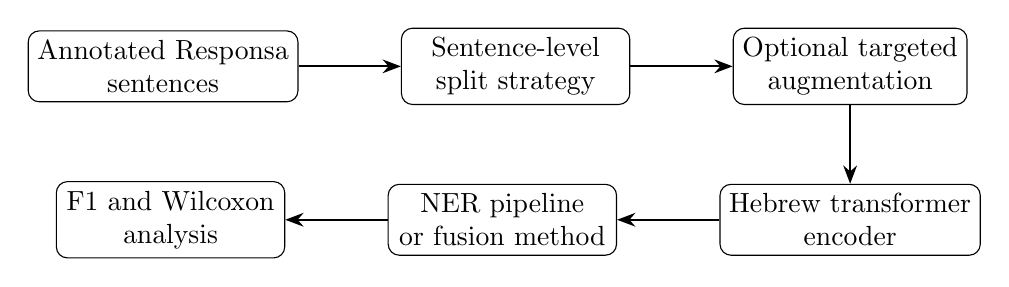
\begin{tikzpicture}[node distance=1.0cm and 1.3cm, box/.style={draw, rounded corners, align=center, minimum width=2.9cm, minimum height=0.85cm}, arr/.style={-{Stealth}, thick}]
\node[box] (data) {Annotated Responsa\\sentences};
\node[box, right=of data] (split) {Sentence-level\\split strategy};
\node[box, right=of split] (aug) {Optional targeted\\augmentation};
\node[box, below=of aug] (models) {Hebrew transformer\\encoder};
\node[box, left=of models] (methods) {NER pipeline\\or fusion method};
\node[box, left=of methods] (eval) {F1 and Wilcoxon\\analysis};
\draw[arr] (data) -- (split);
\draw[arr] (split) -- (aug);
\draw[arr] (aug) -- (models);
\draw[arr] (models) -- (methods);
\draw[arr] (methods) -- (eval);
\end{tikzpicture}
\caption{High-level experimental workflow.}
\label{fig:workflow}
\end{figure}

\section{Sentence-level split strategies}
The dataset is split at sentence level. This avoids leakage where part of a sentence appears in training and another part appears in evaluation. Let the full dataset be
\[
D=\{(x^{(j)},y^{(j)})\}_{j=1}^{N},
\]
where each sentence $x^{(j)}$ has a sequence of token labels $y^{(j)}$. Each split creates disjoint sets
\[
D_{train}^{(c,s)} \cap D_{eval}^{(c,s)} = \emptyset,
\qquad
D_{train}^{(c,s)} \cup D_{eval}^{(c,s)} = D,
\]
with an approximate 70/30 ratio.

\subsection{Baseline random split}
The baseline split shuffles the sentences with seed $s$ and assigns about 70 percent to training and 30 percent to evaluation. This is simple, but it ignores label distribution. With a small imbalanced dataset, rare labels can become poorly represented in one of the splits.

\subsection{Label-aware greedy split}
The label-aware greedy split tries to improve entity coverage in the training set. For a subset $A$ and label $\ell$, define
\[
count_A(\ell)=\sum_{(x,y)\in A}\sum_{i=1}^{|x|}\mathbf{1}[y_i=\ell].
\]
The target training count is approximately
\[
target_{train}(\ell)=0.7\cdot count_D(\ell).
\]
The method greedily selects sentences that reduce the mismatch
\[
\mathcal{L}_{split}(A)=\sum_{\ell\in\mathcal{Y}\setminus\{O\}}\left(count_A(\ell)-target_{train}(\ell)\right)^2.
\]
This method focuses mainly on improving the training set's coverage of non-\texttt{O} labels.

\subsection{Multilabel stratified split}
The multilabel stratified method follows the logic of multilabel stratification \citep{sechidis2011,szymanski2017}. Each sentence is treated as a multilabel item:
\[
L_j=\{\ell:\ell\neq O,\,\ell\text{ appears in sentence }j\}.
\]
For each label $\ell$, the algorithm tracks how many sentences containing that label are still needed in each split. The sentence is assigned to the split with the larger remaining need. This strategy asks which split needs the sentence more in order to preserve the full label distribution.

\section{Targeted masked-language-model augmentation}
Augmentation is applied only to the training set. The evaluation set remains unchanged. This is important because otherwise the test target would also change.

For each entity label $\ell$, let $f(\ell)$ be its frequency in the training set and let
\[
f_{max}=\max_{\ell} f(\ell).
\]
The deficit of label $\ell$ is
\[
\Delta(\ell)=f_{max}-f(\ell).
\]
The number of generated examples is proportional to this deficit:
\[
g(\ell)=r\cdot \Delta(\ell),
\]
with multiplier $r=3$ in the final experiments.

The augmentation uses a masked replacement idea. Given a sentence
\[
x=(w_1,\ldots,w_k,\ldots,w_n),
\]
a relevant entity token is replaced by a mask:
\[
x_{mask}=(w_1,\ldots,[MASK],\ldots,w_n).
\]
The language model estimates
\[
P(w\mid x_{mask})
\]
and a replacement is selected from an entity-compatible vocabulary. The generated sentence preserves the BIO span structure. This follows the general motivation of masked entity augmentation for low-resource NER \citep{zhou2022melm}.

\section{Regular one-stage NER}
The regular NER model uses a transformer encoder followed by a token-classification head. For token $i$, the encoder produces a contextual vector $h_i$. A linear layer produces logits
\[
z_i=Wh_i+b.
\]
The probability of label $k$ is
\[
P(y_i=k\mid x)=\frac{\exp(z_{i,k})}{\sum_{k'\in\mathcal{Y}}\exp(z_{i,k'})}.
\]
The predicted label is
\[
\hat{y}_i=\arg\max_{k\in\mathcal{Y}}P(y_i=k\mid x).
\]
The training objective is token-level cross-entropy over valid tokens:
\[
\mathcal{L}_{NER}=-\sum_{i:y_i\neq -100}\log P(y_i\mid x).
\]

\section{Cascaded three-step NER}
The cascaded method decomposes NER into three tasks: entity detection, BIO boundary prediction, and entity-type prediction. A full label is represented by:
\[
e_i\in\{0,1\},\qquad b_i\in\{B,I\},\qquad t_i\in\mathcal{T}.
\]
For the \texttt{O} label, $e_i=0$ and the boundary and type losses are ignored.

The model has one shared encoder and three heads:
\[
z_i^{entity}=W_eh_i+b_e,
\quad
z_i^{bio}=W_bh_i+b_b,
\quad
z_i^{type}=W_th_i+b_t.
\]
Entity detection and boundary prediction use sigmoid probabilities, while type prediction uses a softmax over entity types. The final label is reconstructed as
\[
\hat{y}_i^{cas}=\begin{cases}
O, & \hat{e}_i=0,\\
\hat{b}_i\text{-}\hat{t}_i, & \hat{e}_i=1.
\end{cases}
\]

The loss combines the three subtasks:
\[
\mathcal{L}_{total}=\mathcal{L}_{entity}+\lambda_{bio}\mathcal{L}_{bio}+\lambda_{type}\mathcal{L}_{type}.
\]
In the implementation, larger weights are assigned to boundary and type prediction because those losses are computed only on entity tokens.

After prediction, two structural repairs are applied. First, an \texttt{I} tag that appears after \texttt{O} or at the start of a sentence is changed to a \texttt{B} tag. Second, if a predicted \texttt{B-X} is followed by \texttt{I-Y} with $X\neq Y$, the inconsistent type is repaired using the stronger probability signal. This keeps the final BIO sequence structurally valid.

\begin{figure}[htbp]
\centering
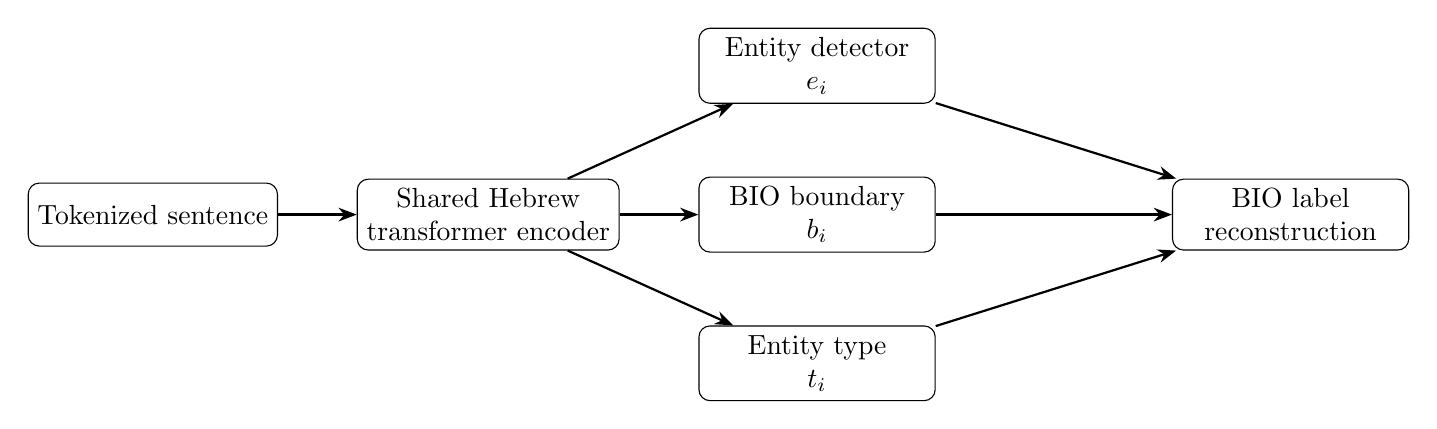
\begin{tikzpicture}[node distance=0.95cm and 1.0cm, box/.style={draw, rounded corners, align=center, minimum width=3.0cm, minimum height=0.8cm}, arr/.style={-{Stealth}, thick}]
\node[box] (input) {Tokenized sentence};
\node[box, right=of input] (enc) {Shared Hebrew\\transformer encoder};
\node[box, above right=of enc] (ent) {Entity detector\\$e_i$};
\node[box, right=of enc] (bio) {BIO boundary\\$b_i$};
\node[box, below right=of enc] (typ) {Entity type\\$t_i$};
\node[box, right=3.0cm of bio] (rec) {BIO label\\reconstruction};
\draw[arr] (input) -- (enc);
\draw[arr] (enc) -- (ent);
\draw[arr] (enc) -- (bio);
\draw[arr] (enc) -- (typ);
\draw[arr] (ent) -- (rec);
\draw[arr] (bio) -- (rec);
\draw[arr] (typ) -- (rec);
\end{tikzpicture}
\caption{Cascaded three-step NER architecture.}
\label{fig:cascade}
\end{figure}

\section{Fusion methods}
Confidence Fusion combines the regular model and the cascaded model. If both systems predict the same label, that label is retained. If they disagree, the label from the more confident system is selected. For token $i$:
\[
\hat{y}_i^{fused}=\begin{cases}
\hat{y}_i^{reg}, & \hat{y}_i^{reg}=\hat{y}_i^{cas},\\
\hat{y}_i^{reg}, & \hat{y}_i^{reg}\neq\hat{y}_i^{cas}\text{ and }p_i^{reg}\geq p_i^{cas},\\
\hat{y}_i^{cas}, & \text{otherwise.}
\end{cases}
\]

SVM Fusion is similar, but it does not use only the raw confidence comparison. It first collects disagreement tokens between the regular and cascaded systems. For training tokens where one of the two systems is correct, a linear SVM learns which source should be trusted. Features include confidence, entropy, probability margin, and disagreement information. The SVM then routes each disagreement token to either the regular or cascaded prediction.

A limitation is important here: in the present experiment, the SVM router is trained from the available ready predictions and is not evaluated on a separate held-out routing split. Therefore, SVM Fusion should be treated as an exploratory router or an upper-bound-style result, not as a fully independent final deployment result. The non-router Confidence Fusion results are more conservative.

\section{Evaluation metrics and statistical tests}
The primary metric is entity-level F1. Precision, recall, and F1 are defined as
\[
Precision=\frac{TP}{TP+FP},
\qquad
Recall=\frac{TP}{TP+FN},
\qquad
F1=\frac{2\cdot Precision\cdot Recall}{Precision+Recall}.
\]
F1 is emphasized because accuracy can be misleading when most tokens are \texttt{O} \citep{sokolova2009,chicco2023mcc}.

For statistical testing, the study uses the paired Wilcoxon signed-rank test. For two methods $A$ and $B$, scores are paired by seed:
\[
d_s=F1_{A,s}-F1_{B,s},\qquad s\in\{1,\ldots,20\}.
\]
The Wilcoxon test checks whether the median paired difference is different from zero. The significance level is $\alpha=0.05$.

\chapter{Results}
\section{One-stage NER and split strategy}
Table~\ref{tab:one_stage_split} shows the one-stage Regular NER results across split strategies. The random split is useful as a baseline, but it is not the most reliable split for this task. The label-aware and multilabel stratified splits generally improve the stability and coverage of entity labels. HeRo is strongest in the one-stage non-augmented setting, while BEREL 3.0 becomes stronger after augmentation in later tables.

\begin{table}[htbp]
\centering
\small
\caption{One-stage NER performance across sentence split strategies. Values are mean entity-level F1 $\pm$ standard deviation over 20 paired seeds.}
\label{tab:one_stage_split}
\begin{tabular}{lcccc}
\toprule
Split strategy & DictaBERT & BEREL 3.0 & HeRo & AlephBERT-Gimmel \\
\midrule
Baseline random & 0.672 $\pm$ 0.011 & 0.705 $\pm$ 0.001 & 0.745 $\pm$ 0.010 & 0.664 $\pm$ 0.001 \\
Label-aware greedy & 0.754 $\pm$ 0.000 & 0.707 $\pm$ 0.000 & 0.755 $\pm$ 0.000 & 0.658 $\pm$ 0.000 \\
Multilabel stratified & 0.738 $\pm$ 0.000 & 0.731 $\pm$ 0.006 & 0.769 $\pm$ 0.000 & 0.627 $\pm$ 0.004 \\
\bottomrule
\end{tabular}
\end{table}

\section{Advanced pipelines without augmentation}
Table~\ref{tab:advanced_nonaug} reports the advanced pipelines without augmentation. The main pattern is that SVM Fusion is the strongest reported method in most non-augmented settings. For example, DictaBERT reaches 0.811 under Label-aware greedy splitting with SVM Fusion, while HeRo reaches 0.805 under Multilabel Stratified splitting with SVM Fusion. However, without augmentation, BEREL 3.0 is not yet clearly dominant.

\begin{landscape}
\begin{table}[htbp]
\centering
\scriptsize
\caption{Advanced pipeline performance without augmentation. Values are mean entity-level F1 $\pm$ standard deviation over 20 paired seeds.}
\label{tab:advanced_nonaug}
\begin{tabular}{llcccc}
\toprule
Split strategy & Method & DictaBERT & BEREL 3.0 & HeRo & AlephBERT-Gimmel \\
\midrule
Baseline random & Regular NER & 0.672 $\pm$ 0.011 & 0.705 $\pm$ 0.001 & 0.745 $\pm$ 0.010 & 0.664 $\pm$ 0.001 \\
 & Cascaded 3-step & 0.737 $\pm$ 0.024 & 0.635 $\pm$ 0.110 & 0.739 $\pm$ 0.028 & 0.690 $\pm$ 0.035 \\
 & Confidence Fusion & 0.686 $\pm$ 0.014 & 0.710 $\pm$ 0.013 & 0.753 $\pm$ 0.012 & 0.691 $\pm$ 0.020 \\
 & SVM Fusion & 0.766 $\pm$ 0.016 & 0.771 $\pm$ 0.025 & 0.795 $\pm$ 0.013 & 0.739 $\pm$ 0.017 \\
\addlinespace[2pt]
Label-aware greedy & Regular NER & 0.754 $\pm$ 0.000 & 0.707 $\pm$ 0.000 & 0.755 $\pm$ 0.000 & 0.658 $\pm$ 0.000 \\
 & Cascaded 3-step & 0.734 $\pm$ 0.028 & 0.652 $\pm$ 0.116 & 0.760 $\pm$ 0.019 & 0.723 $\pm$ 0.025 \\
 & Confidence Fusion & 0.738 $\pm$ 0.011 & 0.715 $\pm$ 0.010 & 0.758 $\pm$ 0.011 & 0.710 $\pm$ 0.022 \\
 & SVM Fusion & 0.811 $\pm$ 0.013 & 0.790 $\pm$ 0.028 & 0.799 $\pm$ 0.012 & 0.763 $\pm$ 0.011 \\
\addlinespace[2pt]
Multilabel stratified & Regular NER & 0.738 $\pm$ 0.000 & 0.731 $\pm$ 0.006 & 0.769 $\pm$ 0.000 & 0.627 $\pm$ 0.004 \\
 & Cascaded 3-step & 0.764 $\pm$ 0.024 & 0.639 $\pm$ 0.147 & 0.750 $\pm$ 0.022 & 0.728 $\pm$ 0.031 \\
 & Confidence Fusion & 0.745 $\pm$ 0.013 & 0.739 $\pm$ 0.012 & 0.776 $\pm$ 0.006 & 0.702 $\pm$ 0.020 \\
 & SVM Fusion & 0.807 $\pm$ 0.010 & 0.795 $\pm$ 0.030 & 0.805 $\pm$ 0.011 & 0.766 $\pm$ 0.015 \\
\addlinespace[2pt]
\bottomrule
\end{tabular}
\end{table}
\end{landscape}

\section{Advanced pipelines with augmentation}
Table~\ref{tab:advanced_aug} shows the same methods after targeted augmentation. The augmented results are substantially higher for most model-method combinations. BEREL 3.0 becomes the strongest model in several settings. The highest numerical mean F1 in the reported results is 0.857 for BEREL 3.0 with baseline random split, augmentation, and SVM Fusion. The strongest robust controlled split setting is 0.852 for BEREL 3.0 with Multilabel Stratified splitting, augmentation, and SVM Fusion. Because the random split is known to be less stable for rare labels, the latter is the preferred main thesis result.

\begin{landscape}
\begin{table}[htbp]
\centering
\scriptsize
\caption{Advanced pipeline performance with targeted augmentation. Values are mean entity-level F1 $\pm$ standard deviation over 20 paired seeds.}
\label{tab:advanced_aug}
\begin{tabular}{llcccc}
\toprule
Split strategy & Method & DictaBERT & BEREL 3.0 & HeRo & AlephBERT-Gimmel \\
\midrule
Baseline random + augmentation & Regular NER & 0.781 $\pm$ 0.011 & 0.836 $\pm$ 0.007 & 0.792 $\pm$ 0.011 & 0.781 $\pm$ 0.008 \\
 & Cascaded 3-step & 0.790 $\pm$ 0.011 & 0.838 $\pm$ 0.010 & 0.796 $\pm$ 0.009 & 0.784 $\pm$ 0.011 \\
 & Confidence Fusion & 0.788 $\pm$ 0.011 & 0.836 $\pm$ 0.009 & 0.785 $\pm$ 0.012 & 0.785 $\pm$ 0.013 \\
 & SVM Fusion & 0.813 $\pm$ 0.012 & 0.857 $\pm$ 0.008 & 0.825 $\pm$ 0.015 & 0.809 $\pm$ 0.010 \\
\addlinespace[2pt]
Label-aware greedy + augmentation & Regular NER & 0.802 $\pm$ 0.011 & 0.824 $\pm$ 0.013 & 0.797 $\pm$ 0.015 & 0.813 $\pm$ 0.010 \\
 & Cascaded 3-step & 0.805 $\pm$ 0.017 & 0.822 $\pm$ 0.007 & 0.785 $\pm$ 0.016 & 0.799 $\pm$ 0.011 \\
 & Confidence Fusion & 0.807 $\pm$ 0.011 & 0.823 $\pm$ 0.011 & 0.787 $\pm$ 0.017 & 0.815 $\pm$ 0.012 \\
 & SVM Fusion & 0.841 $\pm$ 0.013 & 0.844 $\pm$ 0.012 & 0.831 $\pm$ 0.013 & 0.841 $\pm$ 0.012 \\
\addlinespace[2pt]
Multilabel stratified + augmentation & Regular NER & 0.808 $\pm$ 0.010 & 0.847 $\pm$ 0.008 & 0.821 $\pm$ 0.009 & 0.834 $\pm$ 0.006 \\
 & Cascaded 3-step & 0.828 $\pm$ 0.009 & 0.846 $\pm$ 0.008 & 0.825 $\pm$ 0.014 & 0.839 $\pm$ 0.010 \\
 & Confidence Fusion & 0.814 $\pm$ 0.012 & 0.848 $\pm$ 0.008 & 0.823 $\pm$ 0.009 & 0.832 $\pm$ 0.008 \\
 & SVM Fusion & 0.836 $\pm$ 0.008 & 0.852 $\pm$ 0.008 & 0.841 $\pm$ 0.010 & 0.847 $\pm$ 0.008 \\
\addlinespace[2pt]
\bottomrule
\end{tabular}
\end{table}
\end{landscape}

\section{Effect of augmentation}
Table~\ref{tab:augmentation_delta} summarizes the augmentation effect by averaging paired F1 gains over the three split strategies. Augmentation improves all model-method combinations. The largest average gains occur for BEREL 3.0 and AlephBERT-Gimmel, suggesting that augmentation helps especially when the model has room to benefit from better rare-label coverage.

\begin{table}[htbp]
\centering
\small
\caption{Mean F1 gain from targeted augmentation, averaged over the three split strategies. Each value is the paired difference between augmented and non-augmented training for the same model, method, split, and seed.}
\label{tab:augmentation_delta}
\begin{tabular}{lcccc}
\toprule
Method & DictaBERT & BEREL 3.0 & HeRo & AlephBERT-Gimmel \\
\midrule
Regular NER & +0.075 & +0.121 & +0.047 & +0.160 \\
Cascaded 3-step & +0.062 & +0.193 & +0.052 & +0.094 \\
Confidence Fusion & +0.080 & +0.114 & +0.036 & +0.109 \\
SVM Fusion & +0.035 & +0.066 & +0.033 & +0.076 \\
\midrule
Average & +0.063 & +0.123 & +0.042 & +0.110 \\
\bottomrule
\end{tabular}
\end{table}

\begin{figure}[htbp]
\centering
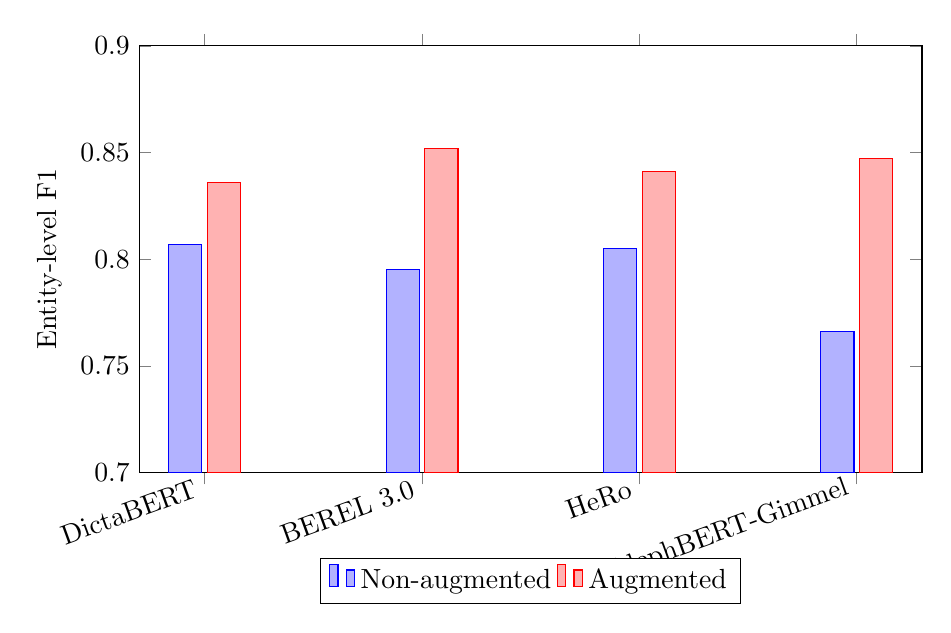
\begin{tikzpicture}
\begin{axis}[
    ybar,
    ymin=0.70,
    ymax=0.90,
    width=0.95\textwidth,
    height=7cm,
    ylabel={Entity-level F1},
    symbolic x coords={DictaBERT,BEREL 3.0,HeRo,AlephBERT-Gimmel},
    xtick=data,
    x tick label style={rotate=20,anchor=east},
    bar width=12pt,
    legend style={at={(0.5,-0.20)},anchor=north,legend columns=2}
]
\addplot coordinates {(DictaBERT,0.807) (BEREL 3.0,0.795) (HeRo,0.805) (AlephBERT-Gimmel,0.766)};
\addplot coordinates {(DictaBERT,0.836) (BEREL 3.0,0.852) (HeRo,0.841) (AlephBERT-Gimmel,0.847)};
\legend{Non-augmented, Augmented}
\end{axis}
\end{tikzpicture}
\caption{SVM Fusion under the Multilabel Stratified split, before and after augmentation.}
\label{fig:svm_multilabel_aug}
\end{figure}

\section{Best configurations and significance tests}
Table~\ref{tab:best_by_model} shows the best mean F1 configuration for each model. All best configurations use augmentation and SVM Fusion. This supports the main conclusion that the largest improvements come from combining stronger data preparation with a fusion-based inference strategy.

\begin{table}[htbp]
\centering
\small
\caption{Best mean F1 configuration for each model among the reported methods.}
\label{tab:best_by_model}
\begin{tabular}{llll}
\toprule
Model & Best method & Split/data condition & F1 \\
\midrule
DictaBERT & SVM Fusion & Label-aware greedy + augmentation & 0.841 $\pm$ 0.013 \\
BEREL 3.0 & SVM Fusion & Baseline random + augmentation & 0.857 $\pm$ 0.008 \\
HeRo & SVM Fusion & Multilabel stratified + augmentation & 0.841 $\pm$ 0.010 \\
AlephBERT-Gimmel & SVM Fusion & Multilabel stratified + augmentation & 0.847 $\pm$ 0.008 \\
\bottomrule
\end{tabular}
\end{table}

Table~\ref{tab:wilcoxon_summary} summarizes the Wilcoxon signed-rank tests. Augmentation improves all 48 paired comparisons and all are significant. Multilabel stratification is especially strong in the augmented setting. SVM Fusion significantly improves over Regular NER and Cascaded 3-step in all tested non-augmented and augmented split combinations, although the SVM router limitation should be remembered when interpreting these results.

\begin{table}[htbp]
\centering
\scriptsize
\caption{Summary of paired Wilcoxon signed-rank tests over seed-aligned runs. Positive means that the first item in the contrast improved F1.}
\label{tab:wilcoxon_summary}
\begin{tabular}{p{4.7cm}p{2.3cm}cccc}
\toprule
Contrast & Setting & Positive & Significant & Mean $\Delta$F1 & Largest $p$ \\
\midrule
Augmentation vs. same split without augmentation & All models, methods, splits & 48/48 & 48/48 & +0.085 & 3.9e-04 \\
Label-aware greedy vs. baseline random & Non-augmented & 14/16 & 10/16 & +0.021 & 0.898 \\
Multilabel stratified vs. baseline random & Non-augmented & 15/16 & 13/16 & +0.024 & 0.927 \\
Label-aware greedy vs. baseline random & Augmented & 11/16 & 13/16 & +0.009 & 0.430 \\
Multilabel stratified vs. baseline random & Augmented & 15/16 & 16/16 & +0.028 & 0.033 \\
SVM Fusion vs. Regular NER & Non-augmented & 12/12 & 12/12 & +0.073 & 8.8e-05 \\
SVM Fusion vs. Cascaded 3-step & Non-augmented & 12/12 & 12/12 & +0.071 & 2.6e-04 \\
SVM Fusion vs. Confidence Fusion & Non-augmented & 12/12 & 12/12 & +0.057 & 9.5e-06 \\
SVM Fusion vs. Regular NER & Augmented & 12/12 & 12/12 & +0.025 & 0.019 \\
SVM Fusion vs. Cascaded 3-step & Augmented & 12/12 & 12/12 & +0.023 & 0.024 \\
SVM Fusion vs. Confidence Fusion & Augmented & 12/12 & 11/12 & +0.025 & 0.076 \\
\bottomrule
\end{tabular}
\end{table}

\section{Interpretation}
The results support four main points. First, a single random split is not enough for a small imbalanced dataset. Even when a random split gives a high numerical score, it may not be the safest basis for conclusions. Second, targeted augmentation consistently improves performance because it increases exposure to rare entity patterns without changing the evaluation set. Third, model choice matters: BEREL 3.0 performs especially well once augmentation and a better split are used, which is consistent with its domain orientation. Fourth, fusion methods are useful because the regular and cascaded systems make different errors.

At the same time, the results should be interpreted carefully. The SVM Fusion method is the strongest reported method, but it is exploratory because the router was not trained on a fully separate routing-development set. The Confidence Fusion result is therefore a more conservative estimate of the benefit of combining regular and cascaded predictions.

\chapter{Comparison with the Closest Work}
The closest recent work is \citet{bengigi2025}. Their study focuses on automatic construction of a citation network from medieval Jewish Responsa literature. It uses sequence labeling and rabbinic-domain BERT-style models to extract references at scale. This thesis shares the same broad goal: automatic extraction of structured references from Responsa literature.

The difference is the level of focus. \citet{bengigi2025} is primarily a large-scale citation-network construction study. This thesis is a controlled low-resource NER methodology study. It asks what should be done when the researcher has only a small annotated dataset, strong class imbalance, and several possible Hebrew encoders. Therefore, the contribution is not simply another extraction system. It is a detailed comparison of data splitting, augmentation, cascaded decomposition, fusion, and statistical testing.

The added value can be summarized as follows:
\begin{enumerate}[leftmargin=*]
\item The thesis isolates the effect of sentence-level split design, showing that label-aware and multilabel splits can change conclusions in small data.
\item It evaluates four Hebrew encoders under the same seed-aligned framework.
\item It tests targeted augmentation for rare reference components.
\item It compares direct token classification with cascaded and fused prediction pipelines.
\item It reports paired Wilcoxon tests over 20 seeds rather than relying only on single-run scores.
\end{enumerate}

This makes the work complementary to \citet{bengigi2025}. A future study should apply the final method to a larger Responsa corpus and compare it directly against a BERT-CRF reference extractor under the same data and label definitions.

\chapter{Limitations and Future Work}
\section{Limitations}
The main limitation is dataset size. With only 300 annotated sentences, even a 20-seed evaluation cannot fully replace a larger independent test set. A second limitation is that entity classes are strongly imbalanced, especially rare prefix classes such as \texttt{pSEC}. A third limitation is that the SVM Fusion router was not trained and evaluated using a fully separate routing split. A fourth limitation is that the experiments do not yet include a direct external comparison against the dataset and system of \citet{bengigi2025}.

The augmentation method also has limits. Synthetic examples can help expose the model to rare labels, but they may also introduce unnatural examples if the replacement is semantically weak. For this reason, augmentation should be inspected manually in future work.

\section{Future work}
A first future direction is to enlarge the annotated corpus. This would make it possible to train a separate development set, test set, and routing set for the SVM Fusion method.

A second direction is to add explicit transition modeling, such as a CRF head or constrained decoding, rather than applying only post-hoc BIO repairs \citep{lafferty2001crf,ma2016}.

A third direction is to add morphological analysis. Hebrew and Aramaic prefixes often carry important information about reference structure. Tools and methods from Hebrew NLP, including the direction discussed by \citet{tsarfaty2019}, could reduce segmentation errors.

A fourth direction is to combine transformer embeddings with stable handcrafted features. For example, quotation marks, abbreviations, prefix markers, and thesaurus matches for tractate or chapter names may help in low-resource conditions. This follows the broader finding that classical features can still be useful for small Hebrew-Aramaic tasks \citep{hacohen2026}.

Finally, the extraction system should be connected to downstream citation-network analysis and citation-intent classification. After references are extracted, one can ask whether a citation is supportive, critical, or neutral \citep{te2022}. This would move the system from reference extraction toward interpretation of halachic authority and disagreement.

\chapter{Conclusion}
This thesis studied reference-component extraction from Hebrew-Aramaic Responsa as a low-resource NER task. The main finding is that performance improves most when several components are combined: domain-relevant Hebrew encoders, careful sentence-level data splitting, targeted augmentation, and fused inference.

The best robust main result is BEREL 3.0 with Multilabel Stratified splitting, targeted augmentation, and SVM Fusion, reaching 0.852 mean F1 over 20 paired seeds. The highest numerical mean in the full result workbook is BEREL 3.0 with baseline random split, augmentation, and SVM Fusion, reaching 0.857, but this setting is less suitable as the main conclusion because random splitting is less reliable for rare labels. A conservative non-router result is BEREL 3.0 with Multilabel Stratified splitting, augmentation, and Confidence Fusion, reaching 0.848.

Overall, the thesis shows that in small specialized Hebrew-Aramaic corpora, the design of the data pipeline is not secondary to model selection. Better splitting, augmentation, and inference design can materially change the final NER result.

\appendix
\chapter{Suggested Figures to Add in the Final Submission}
\placeholder{Add a per-label confusion matrix for the selected robust configuration: BEREL 3.0 + Multilabel Stratified + augmentation + SVM Fusion. This should show which entity types are confused with each other and which are confused with \texttt{O}.}

\placeholder{Add a per-label F1 bar chart for the selected robust configuration. This is important because the overall F1 may hide weak performance on rare labels such as \texttt{pSEC}.}

\placeholder{Add one concrete Hebrew-Aramaic reference example with gold BIO labels and model predictions. This should help non-specialist readers understand what AUT, BOK, pCHP, CHP, pSEC, and SEC mean in real text.}

\chapter{Notes on Reproducibility}
The experiments should be archived with the following items: the final annotated sentence file, the exact train-test split files for all seeds, the augmentation outputs, the model identifiers or local model checkpoints, and the full result workbook. The main reported comparisons require seed-aligned results for all models and methods.


\begin{thebibliography}{99}

\bibitem[Awasthy et~al.(2020)]{awasthy2020}
Awasthy, P., Moon, T., Ni, J., and Florian, R. (2020).
Cascaded models for better fine-grained named entity recognition.
In \emph{Proceedings of EMNLP 2020}, pages 174--184. Association for Computational Linguistics.

\bibitem[Bareket and Tsarfaty(2021)]{bareket2021nemo}
Bareket, D. and Tsarfaty, R. (2021).
Neural modeling for named entities and morphology: NEMO2.
\emph{Transactions of the Association for Computational Linguistics}, 9:909--928.

\bibitem[Beltagy et~al.(2019)]{beltagy2019scibert}
Beltagy, I., Lo, K., and Cohan, A. (2019).
SciBERT: A pretrained language model for scientific text.
In \emph{Proceedings of EMNLP-IJCNLP 2019}, pages 3615--3620.

\bibitem[Ben-Gigi et~al.(2024)]{bengigi2024viewpoint}
Ben-Gigi, N., Zhitomirsky-Geffet, M., Katzoff, B., and Schler, J. (2024).
Citation network analysis for viewpoint plurality assessment of historical corpora: The case of the medieval rabbinic literature.
\emph{PLOS ONE}, 19(7):e0307115.

\bibitem[Ben-Gigi et~al.(2025)]{bengigi2025}
Ben-Gigi, N., Zhitomirsky-Geffet, M., Schler, J., and Katzoff, B. (2025).
Automatic construction of the citation network from the medieval Jewish Responsa literature.
\emph{ACM Journal on Computing and Cultural Heritage}, 18(2):1--18.

\bibitem[Bird et~al.(2009)]{bird2009nltk}
Bird, S., Klein, E., and Loper, E. (2009).
\emph{Natural Language Processing with Python}. O'Reilly Media.

\bibitem[Chicco and Jurman(2023)]{chicco2023mcc}
Chicco, D. and Jurman, G. (2023).
The advantages of the Matthews correlation coefficient over F1 score and accuracy in binary classification evaluation.
\emph{BMC Genomics}, 24:101.

\bibitem[Cohan et~al.(2020)]{cohan2020specter}
Cohan, A., Feldman, S., Beltagy, I., Downey, D., and Weld, D. (2020).
SPECTER: Document-level representation learning using citation-informed transformers.
In \emph{Proceedings of ACL 2020}, pages 2270--2282.

\bibitem[Devlin et~al.(2019)]{devlin2019bert}
Devlin, J., Chang, M.-W., Lee, K., and Toutanova, K. (2019).
BERT: Pre-training of deep bidirectional transformers for language understanding.
In \emph{Proceedings of NAACL-HLT 2019}, pages 4171--4186.

\bibitem[Dietterich(2000)]{dietterich2000}
Dietterich, T. G. (2000).
Ensemble methods in machine learning.
In \emph{Multiple Classifier Systems}, pages 1--15. Springer.

\bibitem[Dinarelli and Rosset(2011)]{dinarelli2011}
Dinarelli, M. and Rosset, S. (2011).
Models cascade for tree-structured named entity detection.
In \emph{Proceedings of IJCNLP 2011}, pages 110--118.

\bibitem[Florian et~al.(2003)]{florian2003}
Florian, R., Ittycheriah, A., Jing, H., and Zhang, T. (2003).
Named entity recognition through classifier combination.
In \emph{Proceedings of CoNLL 2003}, pages 168--171.

\bibitem[Gueta et~al.(2023)]{gueta2023alephgimmel}
Gueta, A., Seker, A., Pereira, L., Neishtadt, E., Bandel, E., Bareket, D., Brusilovsky, I., Greenfeld, R., and Tsarfaty, R. (2023).
Large pre-trained models with extra-large vocabularies: A contrastive analysis of Hebrew BERT models and a new one to outperform them all.
\emph{arXiv:2211.15199}.

\bibitem[HaCohen-Kerner et~al.(2010)]{hacohen2010}
HaCohen-Kerner, Y., Zohar, M., and Mughaz, D. (2010).
Automatic identification of biblical quotations in Hebrew-Aramaic documents.
\emph{Cybernetics and Systems}, 41(3):180--197.

\bibitem[HaCohen-Kerner et~al.(2026)]{hacohen2026}
HaCohen-Kerner, Y., Liskovetsky, K., Mughaz, D., and Miller, D. (2026).
A comparison of advanced machine learning and deep learning methods for short text classification of Hebrew and Aramaic in Jewish Responsa.
\emph{Applied Sciences}, 16(8):3907.

\bibitem[Hu et~al.(2024)]{hu2024ner}
Hu, Q., Yu, G., Wang, X., Fukumoto, F., and Ye, Y. (2024).
A survey on deep learning for named entity recognition.
\emph{IEEE Transactions on Knowledge and Data Engineering}, 36(9):4583--4605.

\bibitem[Itai and Wintner(2008)]{itai2008}
Itai, A. and Wintner, S. (2008).
Language resources for Hebrew.
\emph{Language Resources and Evaluation}, 42:75--98.

\bibitem[Japkowicz and Stephen(2002)]{japkowicz2002}
Japkowicz, N. and Stephen, S. (2002).
The class imbalance problem: A systematic study.
\emph{Intelligent Data Analysis}, 6(5):429--449.

\bibitem[Keraghel et~al.(2024)]{keraghel2024ner}
Keraghel, I., Morbieu, S., and Nadif, M. (2024).
Recent advances in named entity recognition: A comprehensive survey and comparative study.
\emph{arXiv:2401.10825}.

\bibitem[Kohavi(1995)]{kohavi1995}
Kohavi, R. (1995).
A study of cross-validation and bootstrap for accuracy estimation and model selection.
In \emph{Proceedings of IJCAI 1995}, pages 1137--1143.

\bibitem[Lafferty et~al.(2001)]{lafferty2001crf}
Lafferty, J., McCallum, A., and Pereira, F. C. N. (2001).
Conditional random fields: Probabilistic models for segmenting and labeling sequence data.
In \emph{Proceedings of ICML 2001}, pages 282--289.

\bibitem[Li et~al.(2022)]{li2022ner}
Li, J., Sun, A., Han, J., and Li, C. (2022).
A survey on deep learning for named entity recognition.
\emph{IEEE Transactions on Knowledge and Data Engineering}, 34(1):50--70.

\bibitem[Lo et~al.(2020)]{lo2020s2orc}
Lo, K., Wang, L. L., Neumann, M., Kinney, R., and Weld, D. S. (2020).
S2ORC: The Semantic Scholar open research corpus.
In \emph{Proceedings of ACL 2020}, pages 4969--4983.

\bibitem[Ma and Hovy(2016)]{ma2016}
Ma, X. and Hovy, E. (2016).
End-to-end sequence labeling via bi-directional LSTM-CNNs-CRF.
In \emph{Proceedings of ACL 2016}, pages 1064--1074.

\bibitem[Min et~al.(2024)]{min2024plm}
Min, B., Ross, H., Sulem, E., Veyseh, A. P. B., Nguyen, T. H., Sainz, O., Agirre, E., Heinz, I., and Roth, D. (2024).
Recent advances in natural language processing via large pre-trained language models: A survey.
\emph{ACM Computing Surveys}, 56(2):Article 30.

\bibitem[Moghaz et~al.(2019)]{moghaz2019}
Moghaz, D., Zhitomirsky-Geffet, M., and HaCohen-Kerner, Y. (2019).
Text mining for Jewish scholars' birth and death years in Hebrew, Aramaic and Yiddish texts.
\emph{International Journal on Digital Libraries}, 20:197--220.

\bibitem[Mughaz et~al.(2014)]{mughaz2014}
Mughaz, D., HaCohen-Kerner, Y., and Zhitomirsky-Geffet, M. (2014).
Mining and using key-words and key-phrases to identify the era of an anonymous undated Jewish text.
\emph{Journal of Intelligent Information Systems}, 42:285--316.

\bibitem[Nguyen et~al.(2023)]{nguyen2023auc}
Nguyen, N. D., Tan, W., Du, L., Buntine, W., Beare, R., and Chen, C. (2023).
AUC maximization for low-resource named entity recognition.
In \emph{Proceedings of the AAAI Conference on Artificial Intelligence}, 37(11):13389--13399.

\bibitem[Pineau et~al.(2021)]{pineau2021}
Pineau, J., Vincent-Lamarre, P., Sinha, K., Lariviere, V., Beygelzimer, A., d'Alche-Buc, F., Fox, E., and Larochelle, H. (2021).
Improving reproducibility in machine learning research: A report from the NeurIPS 2019 reproducibility program.
\emph{Journal of Machine Learning Research}, 22:1--20.

\bibitem[Ratinov and Roth(2009)]{ratinov2009}
Ratinov, L. and Roth, D. (2009).
Design challenges and misconceptions in named entity recognition.
In \emph{Proceedings of CoNLL 2009}, pages 147--155.

\bibitem[Sade et~al.(2018)]{sade2018}
Sade, S., Seker, A., and Tsarfaty, R. (2018).
The Hebrew Universal Dependency Treebank: Past, present and future.
In \emph{Proceedings of the Second Workshop on Universal Dependencies}, pages 133--143.

\bibitem[Santoso et~al.(2024)]{santoso2024}
Santoso, J., Sutanto, P., Cahyadi, B., and Setiawan, E. (2024).
Pushing the limits of low-resource NER using LLM artificial data generation.
In \emph{Findings of the Association for Computational Linguistics: ACL 2024}.

\bibitem[Satlow and Sperling(2022)]{satlow2022}
Satlow, M. L. and Sperling, M. (2022).
The rabbinic citation network.
\emph{AJS Review}, 46(2):291--319.

\bibitem[Sechidis et~al.(2011)]{sechidis2011}
Sechidis, K., Tsoumakas, G., and Vlahavas, I. (2011).
On the stratification of multi-label data.
In \emph{Proceedings of ECML PKDD 2011}, pages 145--158. Springer.

\bibitem[Seker et~al.(2022)]{seker2022alephbert}
Seker, A., Bandel, E., Bareket, D., Brusilovsky, I., Greenfeld, R., and Tsarfaty, R. (2022).
AlephBERT: Language model pre-training and evaluation from sub-word to sentence level.
In \emph{Proceedings of ACL 2022}, pages 46--56.

\bibitem[Shalumov and Haskey(2023)]{shalumov2023hero}
Shalumov, V. and Haskey, H. (2023).
HeRo: RoBERTa and Longformer Hebrew language models.
\emph{arXiv:2304.11077}.

\bibitem[Shmidman et~al.(2022)]{shmidman2022berel}
Shmidman, A., Guedalia, J., Shmidman, S., Shmidman, C. S., Handel, E., and Koppel, M. (2022).
BEREL: BERT embeddings for rabbinic-encoded language.
In \emph{Proceedings of the Workshop on Language Technologies for Historical and Ancient Languages}, pages 49--54.

\bibitem[Shmidman et~al.(2023)]{shmidman2023dictabert}
Shmidman, A., Shmidman, S., and Koppel, M. (2023).
DictaBERT: A state-of-the-art BERT suite for Modern Hebrew.
\emph{arXiv:2308.16687}.

\bibitem[Sokolova and Lapalme(2009)]{sokolova2009}
Sokolova, M. and Lapalme, G. (2009).
A systematic analysis of performance measures for classification tasks.
\emph{Information Processing and Management}, 45(4):427--437.

\bibitem[Szymanski and Kajdanowicz(2017)]{szymanski2017}
Szymanski, P. and Kajdanowicz, T. (2017).
A network perspective on stratification of multi-label data.
In \emph{Proceedings of LID 2017}, pages 22--35. PMLR.

\bibitem[Te et~al.(2022)]{te2022}
Te, S., Barhoumi, A., Lentschat, M., Bordignon, F., Labbe, C., and Portet, F. (2022).
Citation context classification: Critical vs. non-critical.
In \emph{Proceedings of the Third Workshop on Scholarly Document Processing}, pages 49--53.

\bibitem[Tsarfaty et~al.(2019)]{tsarfaty2019}
Tsarfaty, R., Sadde, S., Klein, S., and Seker, A. (2019).
What's wrong with Hebrew NLP? and how to make it right.
In \emph{Proceedings of EMNLP-IJCNLP: System Demonstrations}, pages 259--264.

\bibitem[Webster and Kit(1992)]{webster1992}
Webster, J. J. and Kit, C. (1992).
Tokenization as the initial phase in NLP.
In \emph{Proceedings of COLING 1992}, pages 1106--1110.

\bibitem[Wei and Zou(2019)]{wei2019eda}
Wei, J. and Zou, K. (2019).
EDA: Easy data augmentation techniques for boosting performance on text classification.
In \emph{Proceedings of EMNLP-IJCNLP 2019}, pages 6382--6388.

\bibitem[Zhao et~al.(2023)]{zhao2023llm}
Zhao, W. X., Zhou, K., Li, J., Tang, T., Wang, X., Hou, Y., Min, Y., Zhang, B., Zhang, J., Dong, Z., Du, Y., Yang, C., Chen, Y., Chen, Z., Jiang, J., Ren, R., Li, Y., Tang, X., Liu, Z., Liu, P., Nie, J.-Y., and Wen, J.-R. (2023).
A survey of large language models.
\emph{arXiv:2303.18223}.

\bibitem[Zhou et~al.(2022)]{zhou2022melm}
Zhou, R., Li, X., He, R., Bing, L., Cambria, E., and Miao, C. (2022).
MELM: Data augmentation with masked entity language modeling for low-resource NER.
In \emph{Proceedings of ACL 2022}, pages 2246--2261.

\end{thebibliography}


\end{document}
